% ----------------------------------------------------------
% Apêndices
% Documentos gerados pelo próprio autor
% ----------------------------------------------------------

% ---
% Inicia os apêndices
% ---
\begin{apendicesenv}

% Imprime uma página indicando o início dos apêndices
\partapendices

% ----------------------------------------------------------
\chapter{Publicações do Blog}
% ----------------------------------------------------------

\begin{figure}[H]
	\centering
	\caption{Blog: Apresentação}
	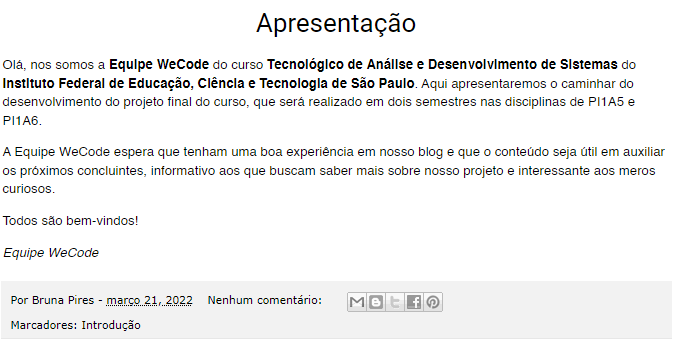
\includegraphics[width=0.95\textwidth]{../imagens/blog-posts/semana00apresentacao.png}
\end{figure}

\begin{figure}[H]
	\centering
	\caption{Blog: Semana 1}
	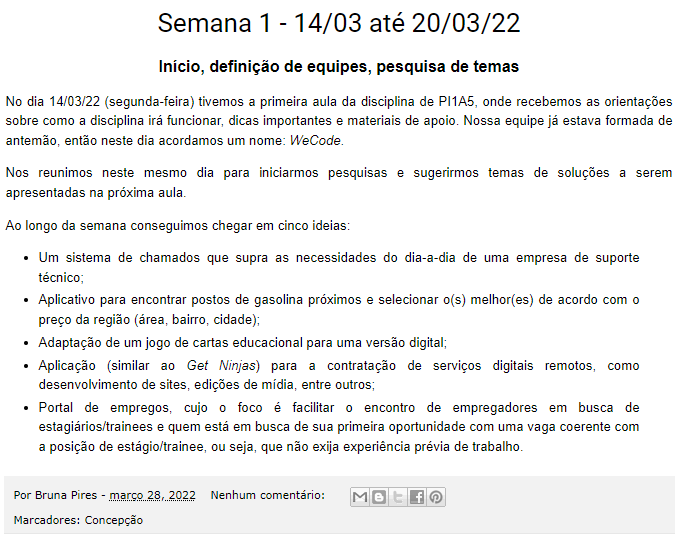
\includegraphics[width=0.95\textwidth]{../imagens/blog-posts/semana01.png}
\end{figure}
\begin{figure}[H]
	\centering
	\caption{Blog: Semana 2}
	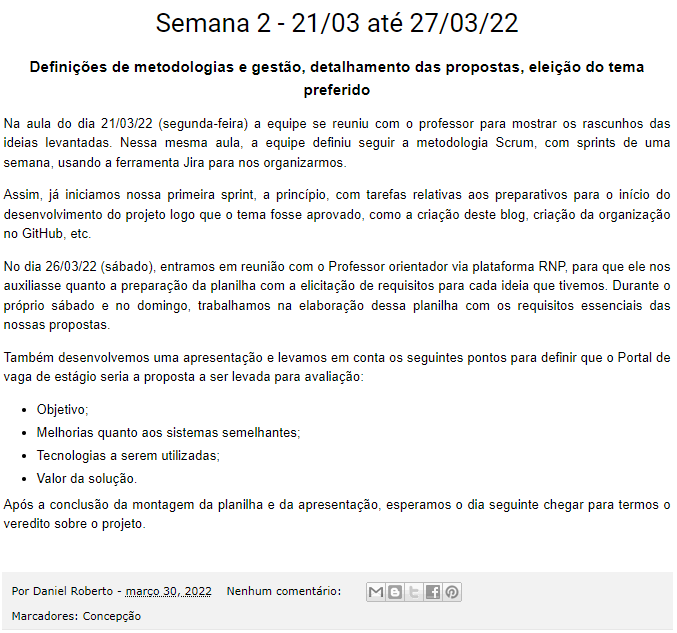
\includegraphics[width=0.95\textwidth]{../imagens/blog-posts/semana02.png}
\end{figure}
\begin{figure}[H]
	\centering
	\caption{Blog: Semana 3}
	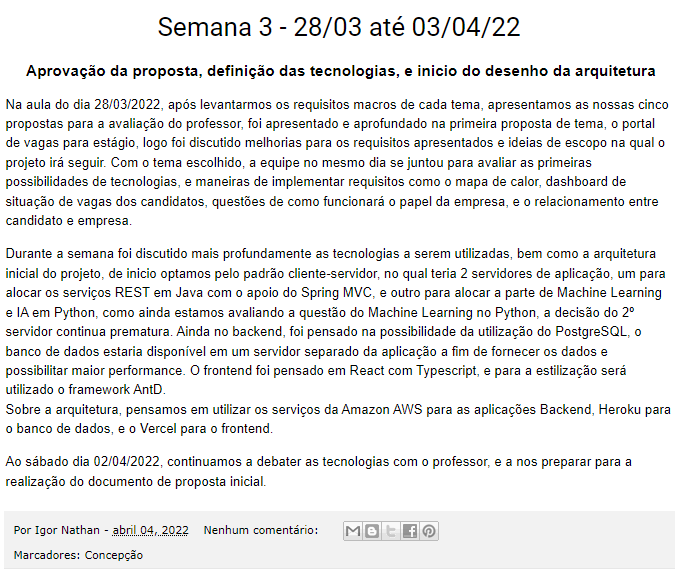
\includegraphics[width=0.95\textwidth]{../imagens/blog-posts/semana03.png}
\end{figure}
\begin{figure}[H]
	\centering
	\caption{Blog: Semana 4}
	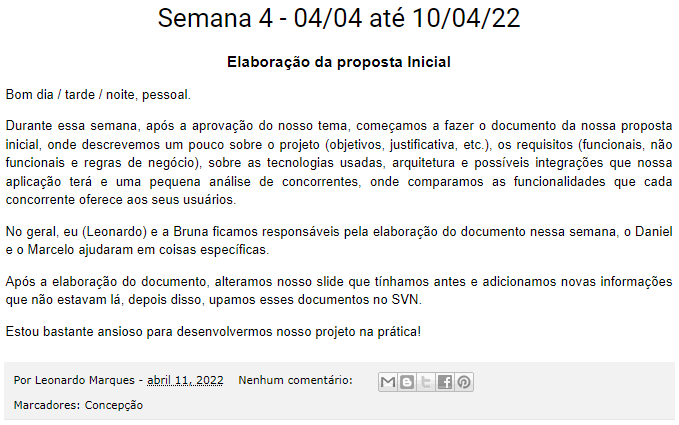
\includegraphics[width=0.95\textwidth]{../imagens/blog-posts/semana04.png}
\end{figure}
\begin{figure}[H]
	\centering
	\caption{Blog: Semana 5}
	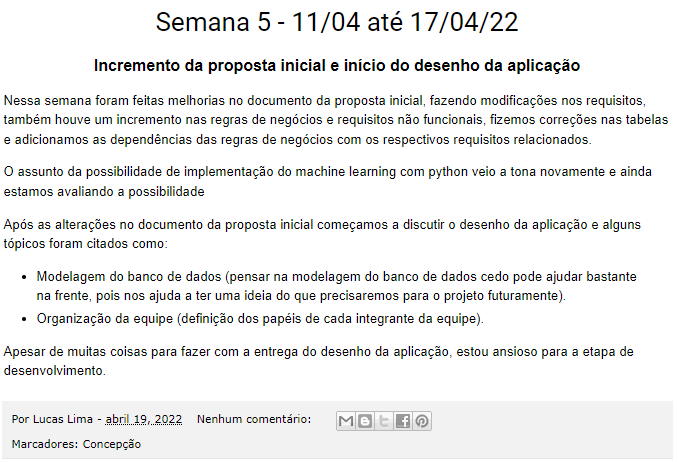
\includegraphics[width=0.95\textwidth]{../imagens/blog-posts/semana05.png}
\end{figure}
\begin{figure}[H]
	\centering
	\caption{Blog: Semana 6}
	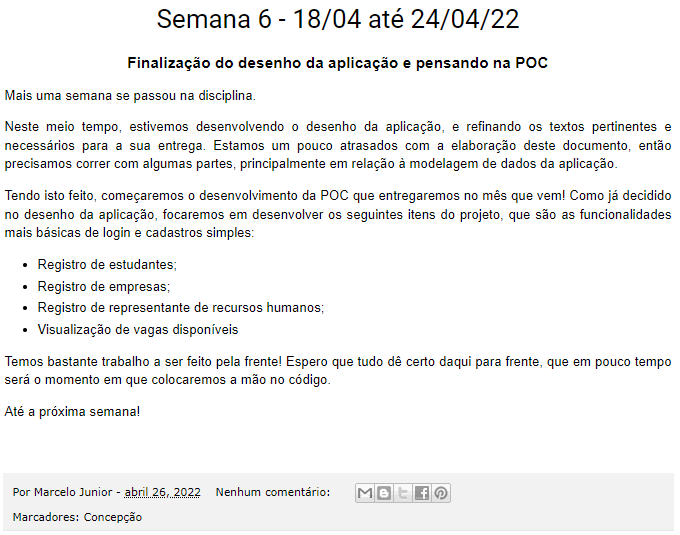
\includegraphics[width=0.95\textwidth]{../imagens/blog-posts/semana06.png}
\end{figure}
\begin{figure}[H]
	\centering
	\caption{Blog: Semana 7 - 1}
	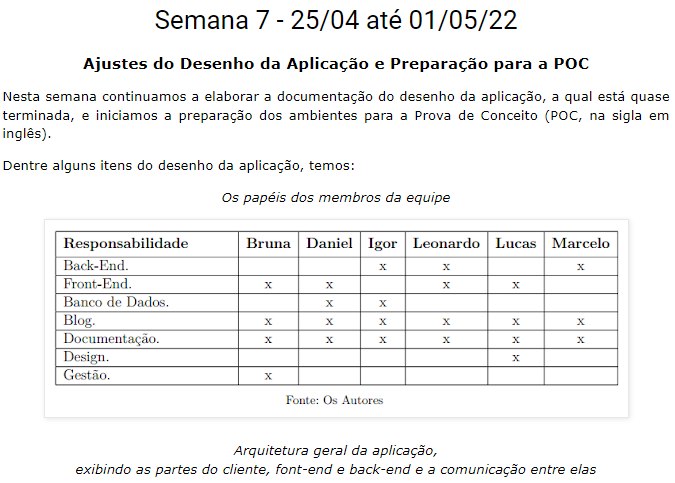
\includegraphics[width=0.95\textwidth]{../imagens/blog-posts/semana07-1.png}
\end{figure}
\begin{figure}[H]
	\centering
	\caption{Blog: Semana 7 - 2}
	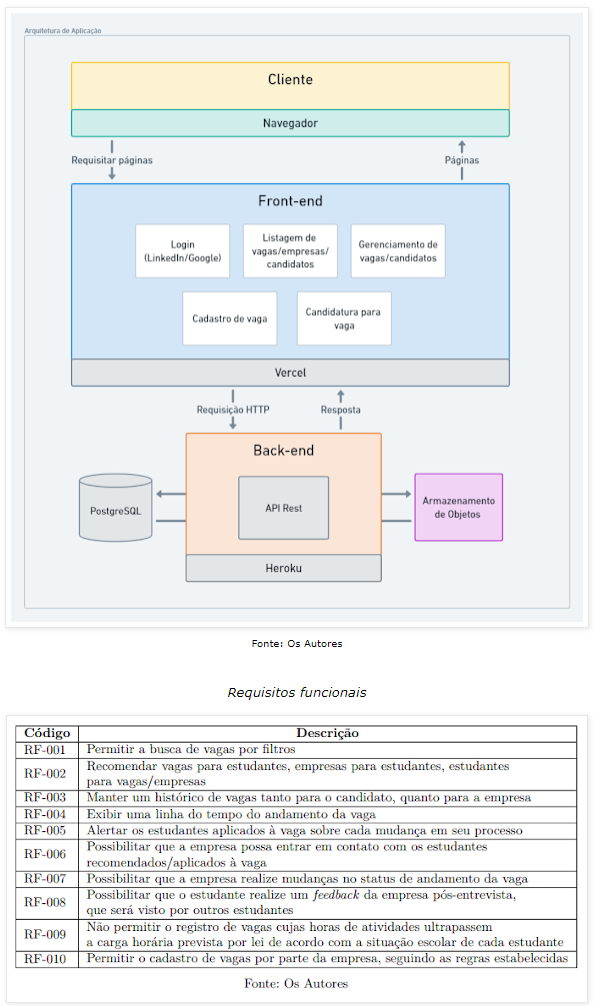
\includegraphics[width=0.9\textwidth]{../imagens/blog-posts/semana07-2.png}
\end{figure}
\begin{figure}[H]
	\centering
	\caption{Blog: Semana 7 - 3}
	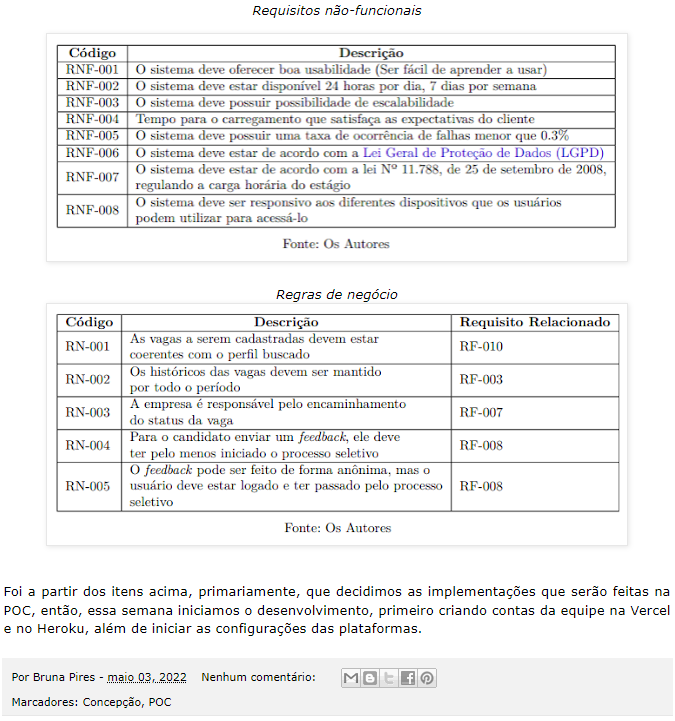
\includegraphics[width=0.95\textwidth]{../imagens/blog-posts/semana07-3.png}
\end{figure}
\begin{figure}[H]
	\centering
	\caption{Blog: Semana 8 - 1}
	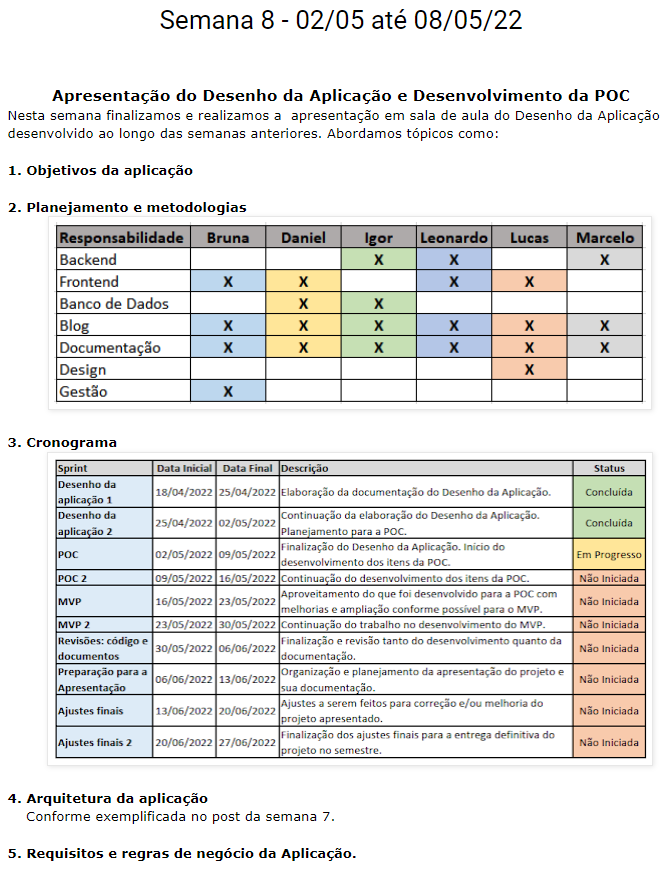
\includegraphics[width=0.95\textwidth]{../imagens/blog-posts/semana08-1.png}
\end{figure}
\begin{figure}[H]
	\centering
	\caption{Blog: Semana 8 - 2}
	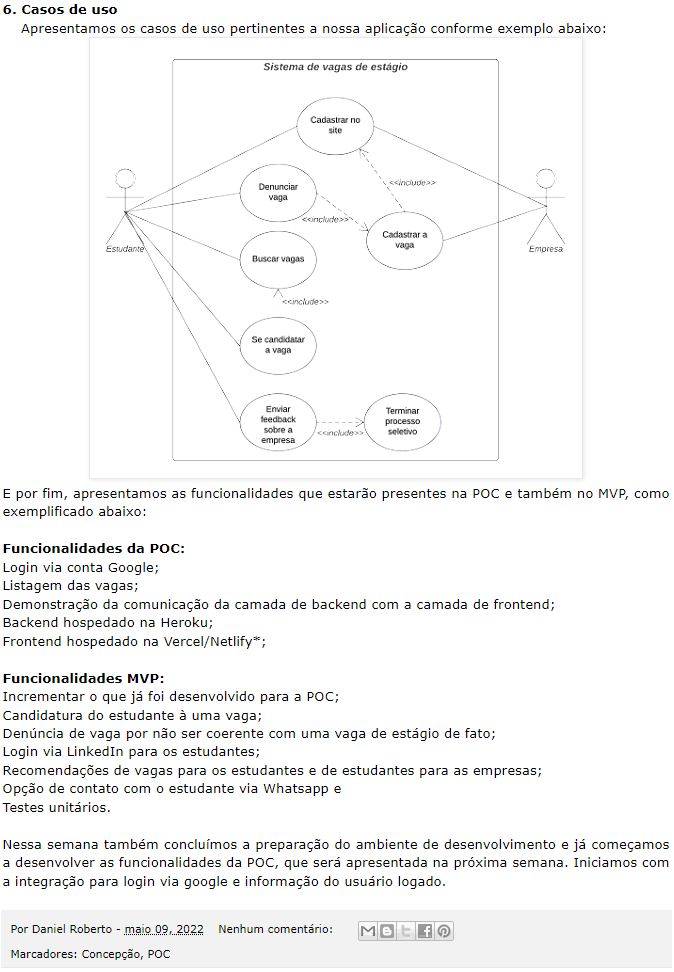
\includegraphics[width=0.95\textwidth]{../imagens/blog-posts/semana08-2.png}
\end{figure}
\begin{figure}[H]
	\centering
	\caption{Blog: Semana 9 - 1}
	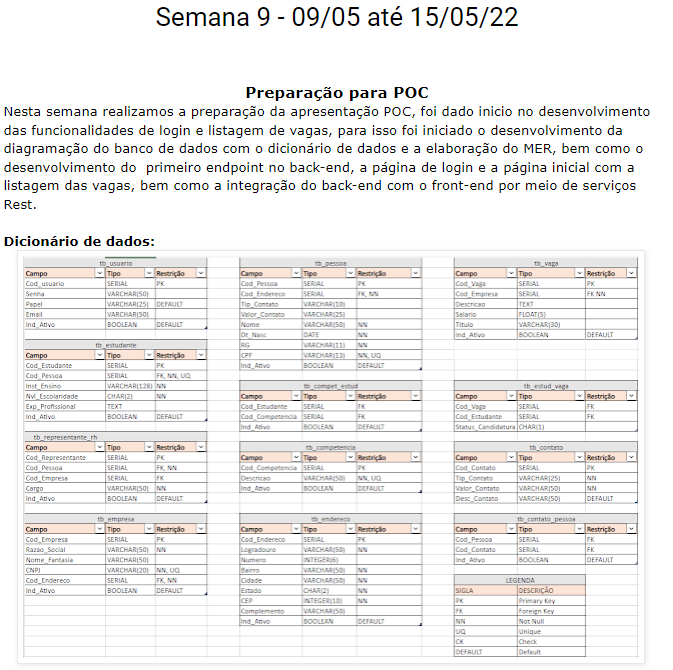
\includegraphics[width=0.95\textwidth]{../imagens/blog-posts/semana09-1.png}
\end{figure}
\begin{figure}[H]
	\centering
	\caption{Blog: Semana 9 - 2}
	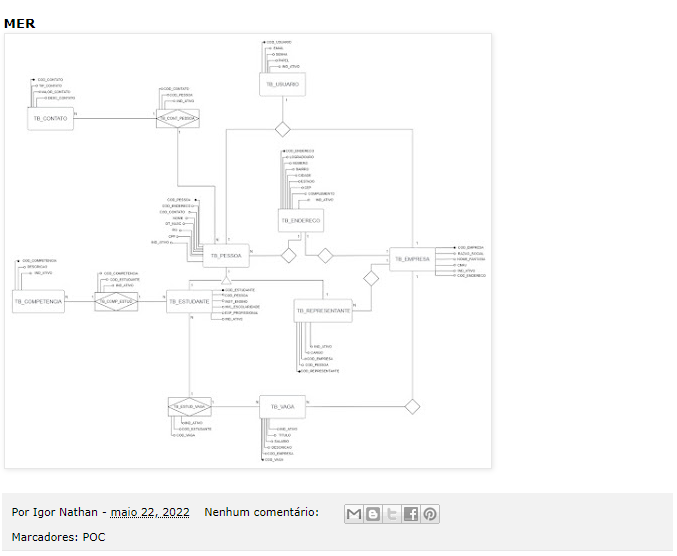
\includegraphics[width=0.95\textwidth]{../imagens/blog-posts/semana09-2.png}
\end{figure}
\begin{figure}[H]
	\centering
	\caption{Blog: Semana 10}
	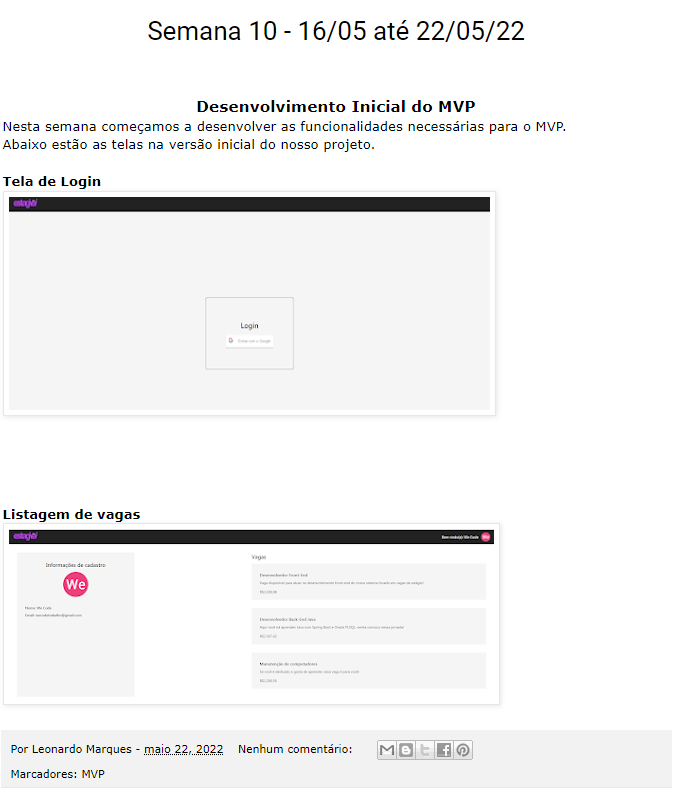
\includegraphics[width=0.95\textwidth]{../imagens/blog-posts/semana10.png}
\end{figure}
\begin{figure}[H]
	\centering
	\caption{Blog: Semana 11}
	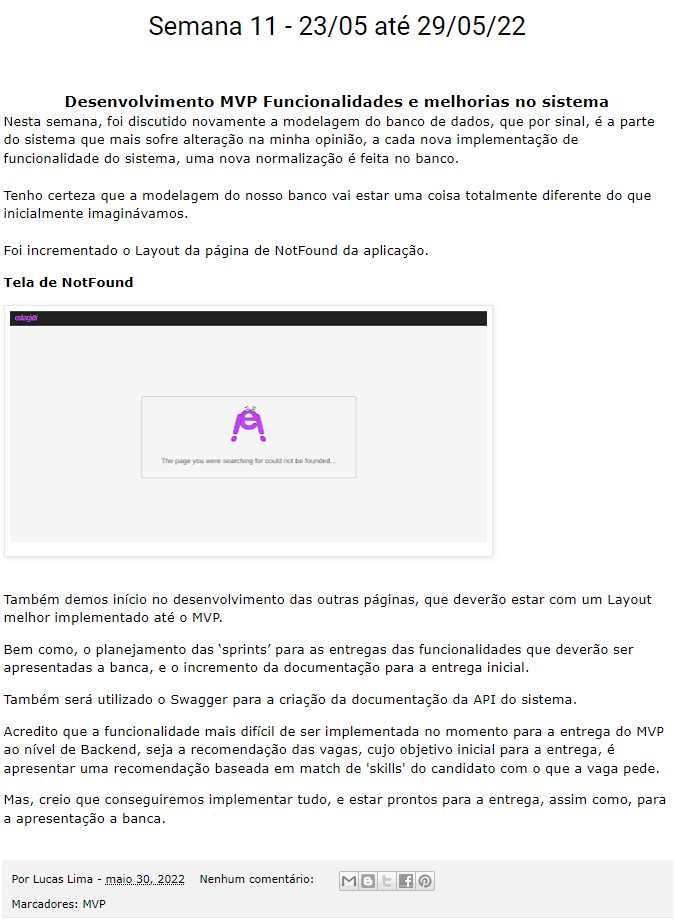
\includegraphics[width=0.95\textwidth]{../imagens/blog-posts/semana11.png}
\end{figure}
\begin{figure}[H]
	\centering
	\caption{Blog: Semana 12}
	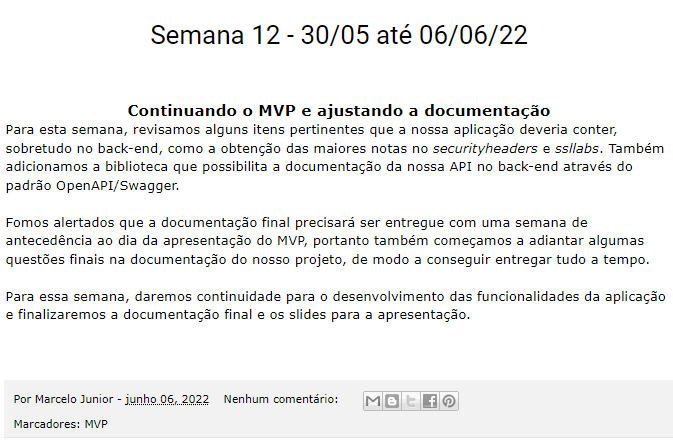
\includegraphics[width=0.95\textwidth]{../imagens/blog-posts/semana12.png}
\end{figure}

% ----------------------------------------------------------
\chapter{Desenho da Aplicação}
% ----------------------------------------------------------


\end{apendicesenv}
% ---
